%%%%%%%%%%%%%%%%%%%%%%%%%%%%%%%%%%%%%%%%%%%%%%%%%%%%%%%%%%%%%%
\chapter{ProSiT Model Inventory}
\label{app:prosit_inventory}
%%%%%%%%%%%%%%%%%%%%%%%%%%%%%%%%%%%%%%%%%%%%%%%%%%%%%%%%%%%%%%
% Sources (trucksimulation): simulation_e3/runs/hm07orig_20261115/make_inventory_appendix.py
%   (tables/app_inventory.tex, model_leaves.csv, model_inventory.csv); export_simulation_model.py (Chapter 5 tables);
%   plot_control_flow.py (net figures); data/processed/CTB/split13apr_20261106/manifest.json (hashes).

This appendix lists everything needed to set up the final simulation model with
ProSiT: the settings and inputs, every learned model, the capacities and
calendars, the domain rules and the discovered nets. Chapter~\ref{chp:process_discovery_methodology}
shows and interprets the most important trees; Section~\ref{sec:res_inspection}
discusses whether their features and targets are plausible for the terminal.

\section{Settings, Versions and Inputs}
\label{app:prosit_settings}

The model is discovered with ProSiT~1.0.4 (\texttt{prosit-pm}) on PM4Py
2.7.22.3 and Python 3.11, with the settings of
Tables~\ref{tab:sim_hyperparameters} and~\ref{tab:exp_e3_config}: trees of depth
at most three, at least 50, 100 or 200 cases per leaf chosen by five-fold
cross-validation with the continuous ranked probability score, the planned
manifest as case attributes, workload features and multitasking on, and random
state 42. The inputs are the net HM 0.7 as exported from ProM with its initial and
final marking, and the training log of 59,139 visits (2 March to 11 April 2026,
SHA-256 \texttt{58932826\ldots 6cb94b}). The test log has 32,014 visits (13 to 30
April 2026, SHA-256 \texttt{dee4cb78\ldots 4cda30}). The four adaptations of
Table~\ref{tab:sim_adaptations} are switches in the simulation loop; the final
configuration sets all of them. Every configuration of E3 and E4 is run with seeds
42 to 46, E5 with seeds 42 to 51.

\section{Learned Models}
\label{app:prosit_trees}

Table~\ref{tab:app_inventory} lists every learned model of the final model: the
arrival tree, the routing model of every transition of HM 0.7, the waiting-time
model of every resource (lane-free target) and the execution-time model of every
activity (with the trucks at the block as a feature). The learned block choice is
listed as well, although the final configuration replays the observed blocks. A
routing transition is named by its identifier in the PNML file and, for a silent
transition, by the step it stands for. The file \texttt{model\_leaves.csv} of the
reproduction package gives every one of the 481 leaves with its path of splits,
its fitted distribution and parameters, its mean or firing probability and its
sample size.

\begin{longtable}{L{4.2cm}L{1.6cm}rrL{4.0cm}L{1.9cm}}
\caption{Every learned model of the final simulation model. Leaves: number of leaves; range: smallest and largest leaf mean (minutes) or firing probability (routing). Every leaf with its distribution, parameters and sample size is listed in \texttt{model\_leaves.csv} of the reproduction package.}\label{tab:app_inventory}\\
\toprule
\textbf{Model} & \textbf{Form} & \textbf{Depth} & \textbf{Leaves} & \textbf{Split features} & \textbf{Range} \\
\midrule
\endfirsthead
\toprule
\textbf{Model} & \textbf{Form} & \textbf{Depth} & \textbf{Leaves} & \textbf{Split features} & \textbf{Range} \\
\midrule
\endhead
\bottomrule
\endfoot
\multicolumn{6}{l}{\textit{Arrivals}} \\
arrivals & tree & 3 & 7 & hour, weekday & 0.533 -- 34.6 \\
\multicolumn{6}{l}{\textit{Routing}} \\
n52: Gate In & constant & 0 & 1 &  & 1 \\
n43: Gate In $\rightarrow$ LL\_delivery & tree & 3 & 8 & deliveries, flow type, full ratio, planned stops, visit complexity & 0 -- 0.864 \\
n25: Gate In $\rightarrow$ RMG\_mixed & tree & 3 & 7 & flow type, planned stops, visit complexity & 0 -- 0.87 \\
n36: Gate In $\rightarrow$ HO2\_mixed & tree & 3 & 8 & planned stops, reefer, visit complexity & 0 -- 0.702 \\
n37: Gate In $\rightarrow$ LL\_mixed & tree & 3 & 5 & containers, full ratio, visit complexity & 0 -- 0.271 \\
n60: Gate In $\rightarrow$ RMG\_receive & tree & 3 & 7 & flow type, full ratio, planned stops, visit complexity & 0 -- 0.879 \\
n51: Gate In $\rightarrow$ HO2\_delivery & tree & 3 & 7 & containers, flow type, full ratio, planned stops, visit complexity & 0 -- 1 \\
n26: Gate In $\rightarrow$ RMG\_delivery & tree & 3 & 7 & flow type, full ratio, planned stops, visit complexity & 0 -- 0.754 \\
n67: Gate In $\rightarrow$ HO2\_receive & tree & 3 & 7 & flow type, hazardous, planned stops, visit complexity & 0 -- 0.311 \\
n56: Gate In $\rightarrow$ LL\_receive & tree & 3 & 7 & deliveries, flow type, full ratio, planned stops, receives & 0 -- 0.69 \\
n65: RMG\_delivery & constant & 0 & 1 &  & 1 \\
n44: RMG\_delivery $\rightarrow$ Gate Out & tree & 1 & 2 & flow type & 0.012 -- 0.994 \\
n40: RMG\_delivery $\rightarrow$ LL\_receive & tree & 2 & 3 & flow type, full ratio & 0 -- 0.453 \\
n32: RMG\_delivery $\rightarrow$ HO2\_receive & tree & 1 & 2 & visit complexity & 0 -- 0.067 \\
n35: RMG\_delivery $\rightarrow$ RMG\_receive & tree & 2 & 3 & flow type, full ratio & 0 -- 0.959 \\
n57: RMG\_delivery $\rightarrow$ RMG\_delivery & tree & 3 & 5 & activity done, containers, deliveries, visit complexity & 0 -- 0.571 \\
n62: Gate Out & constant & 0 & 1 &  & 1 \\
n27: RMG\_receive & constant & 0 & 1 &  & 1 \\
n47: RMG\_receive $\rightarrow$ RMG\_receive & tree & 2 & 3 & activity done, receives & 0 -- 0.264 \\
n38: RMG\_receive $\rightarrow$ Gate Out & tree & 2 & 3 & activity done, receives & 0.736 -- 1 \\
n33: LL\_delivery & constant & 0 & 1 &  & 1 \\
n34: LL\_delivery $\rightarrow$ HO2\_mixed & tree & 2 & 3 & full ratio, visit complexity & 0 -- 0.086 \\
n29: LL\_delivery $\rightarrow$ RMG\_delivery & tree & 3 & 4 & deliveries, planned stops, visit complexity & 0 -- 0.899 \\
n41: LL\_delivery $\rightarrow$ RMG\_receive & tree & 3 & 5 & flow type, receives, visit complexity & 0 -- 0.96 \\
n55: LL\_delivery $\rightarrow$ Gate Out & tree & 3 & 4 & full ratio, planned stops, visit complexity & 0.002 -- 1 \\
n63: LL\_delivery $\rightarrow$ HO2\_receive & tree & 2 & 3 & flow type, visit complexity & 0 -- 0.117 \\
n50: LL\_delivery $\rightarrow$ RMG\_mixed & tree & 3 & 6 & deliveries, full ratio, planned stops, visit complexity & 0 -- 0.952 \\
n54: HO2\_delivery & constant & 0 & 1 &  & 1 \\
n49: HO2\_delivery $\rightarrow$ LL\_receive & tree & 2 & 3 & flow type, full ratio & 0 -- 0.327 \\
n23: HO2\_delivery $\rightarrow$ RMG\_receive & tree & 1 & 2 & flow type & 0 -- 0.89 \\
n39: HO2\_delivery $\rightarrow$ Gate Out & tree & 1 & 2 & flow type & 0.011 -- 1 \\
n24: HO2\_receive & constant & 0 & 1 &  & 1 \\
n59: HO2\_receive $\rightarrow$ Gate Out & tree & 1 & 2 & receives & 0.667 -- 0.997 \\
n58: HO2\_receive $\rightarrow$ HO2\_receive & tree & 1 & 2 & receives & 0.003 -- 0.333 \\
n53: RMG\_mixed & constant & 0 & 1 &  & 1 \\
n45: RMG\_mixed $\rightarrow$ RMG\_receive & tree & 3 & 4 & deliveries, planned stops, receives & 0 -- 0.895 \\
n66: RMG\_mixed $\rightarrow$ Gate Out & tree & 3 & 4 & deliveries, planned stops, receives & 0.105 -- 1 \\
n48: HO2\_mixed & constant & 0 & 1 &  & 1 \\
n64: HO2\_mixed $\rightarrow$ Gate Out & constant & 0 & 1 &  & 1 \\
n46: LL\_receive & constant & 0 & 1 &  & 1 \\
n28: LL\_receive $\rightarrow$ RMG\_receive & tree & 2 & 3 & full ratio, receives & 0 -- 0.908 \\
n42: LL\_receive $\rightarrow$ Gate Out & tree & 2 & 3 & full ratio, receives & 0.092 -- 1 \\
n31: LL\_mixed & constant & 0 & 1 &  & 1 \\
n30: LL\_mixed $\rightarrow$ Gate Out & tree & 1 & 2 & visit complexity & 0 -- 1 \\
n61: LL\_mixed $\rightarrow$ RMG\_receive & tree & 1 & 2 & visit complexity & 0 -- 1 \\
\multicolumn{6}{l}{\textit{Block choice (not used in the final configuration)}} \\
HO2 & tree & 1 & 2 & queue length & 0.222 -- 0.997 \\
LL & tree & 3 & 5 & deliveries, full ratio, queue length, receives & 0 -- 1 \\
Res.GateIn & constant & 0 & 1 &  & 1 \\
Res.GateOut & tree & 3 & 8 & block, deliveries, planned stops, receives, visit complexity & 0 -- 1 \\
T06 & tree & 3 & 5 & block, planned stops, queue length, visit complexity & 0 -- 0.305 \\
T07 & tree & 1 & 2 & queue length & 0 -- 0.102 \\
T08 & tree & 2 & 3 & queue length, workload & 0 -- 0.113 \\
T09 & tree & 2 & 3 & queue length, workload & 0 -- 0.112 \\
T10 & tree & 2 & 3 & queue length, workload & 0 -- 0.141 \\
T11 & tree & 3 & 5 & queue length, reefer, workload & 0 -- 0.256 \\
T12 & tree & 2 & 3 & queue length, workload & 0 -- 0.118 \\
T13 & tree & 2 & 3 & queue length, workload & 0 -- 0.127 \\
T14 & tree & 2 & 3 & queue length, workload & 0 -- 0.128 \\
T15 & tree & 3 & 5 & full ratio, queue length, reefer, workload & 0 -- 0.256 \\
T16 & tree & 3 & 5 & queue length, reefer, visit complexity, workload & 0 -- 0.14 \\
T17 & tree & 3 & 7 & flow type, full ratio, queue length, reefer, workload & 0 -- 0.238 \\
T18 & tree & 3 & 5 & activity, queue length, workload & 0 -- 0.16 \\
T19 & tree & 2 & 3 & queue length, reefer & 0 -- 0.217 \\
T20 & tree & 3 & 5 & queue length, workload & 0 -- 0.147 \\
T21 & tree & 3 & 5 & queue length, workload & 0 -- 0.15 \\
T22 & tree & 3 & 5 & queue length, workload & 0 -- 0.146 \\
T23 & tree & 3 & 5 & queue length, visit complexity, workload & 0 -- 0.134 \\
T24 & tree & 3 & 5 & queue length, reefer, workload & 0 -- 0.135 \\
T25 & tree & 2 & 3 & queue length, reefer & 0 -- 0.204 \\
T26 & tree & 1 & 2 & queue length & 0 -- 0.094 \\
T27 & tree & 3 & 5 & activity, full ratio, queue length, reefer & 0 -- 0.24 \\
\multicolumn{6}{l}{\textit{Waiting time (lane-free target)}} \\
HO2 & tree & 3 & 8 & hour, queue length, workload & 8.38 -- 84.1 \\
LL & tree & 3 & 5 & queue length, workload & 6.1 -- 41.2 \\
Res.GateIn & single distribution & 0 & 1 &  & 0 \\
Res.GateOut & tree & 3 & 8 & flow type, hour, queue length & 9.49 -- 118 \\
T06 & tree & 3 & 7 & queue length & 6.55 -- 39.2 \\
T07 & tree & 3 & 6 & queue length, workload & 6.31 -- 42.5 \\
T08 & tree & 3 & 6 & queue length, workload & 6.34 -- 73.9 \\
T09 & tree & 3 & 7 & queue length, workload & 6.46 -- 34.9 \\
T10 & tree & 3 & 4 & queue length & 6.43 -- 76.6 \\
T11 & tree & 3 & 7 & queue length, workload & 6.77 -- 63.5 \\
T12 & tree & 3 & 6 & queue length, visit complexity, workload & 6.33 -- 22.7 \\
T13 & tree & 3 & 6 & activity, queue length & 7.09 -- 101 \\
T14 & tree & 3 & 5 & queue length, workload & 6.59 -- 44.4 \\
T15 & tree & 3 & 6 & queue length, weekday, workload & 6.65 -- 35.6 \\
T16 & tree & 3 & 7 & flow type, queue length & 6.56 -- 55.6 \\
T17 & tree & 3 & 8 & queue length, visit complexity, workload & 7.25 -- 41.2 \\
T18 & tree & 3 & 7 & queue length, workload & 4.96 -- 51.8 \\
T19 & tree & 3 & 7 & hour, queue length, visit complexity & 7.12 -- 35.1 \\
T20 & tree & 3 & 6 & queue length, workload & 6.64 -- 35.2 \\
T21 & tree & 3 & 6 & hour, queue length, weekday, workload & 5.9 -- 18.1 \\
T22 & tree & 3 & 6 & activity done, hour, queue length & 6.85 -- 19.1 \\
T23 & tree & 3 & 6 & deliveries, queue length, workload & 6.83 -- 19 \\
T24 & tree & 3 & 7 & hour, queue length, workload & 5.31 -- 22.5 \\
T25 & tree & 3 & 5 & queue length, weekday, workload & 8.44 -- 35.8 \\
T26 & tree & 3 & 5 & queue length, workload & 8 -- 57.8 \\
T27 & tree & 3 & 6 & queue length, weekday, workload & 8.39 -- 45.1 \\
\multicolumn{6}{l}{\textit{Execution time (with load)}} \\
Gate In & single distribution & 0 & 1 &  & 0 \\
Gate Out & tree & 3 & 4 & block, trucks at block at start & 0 -- 17.2 \\
HO2\_delivery & tree & 3 & 6 & hour, trucks at block at start & 6.68 -- 25.9 \\
HO2\_mixed & tree & 3 & 6 & full ratio, hour, trucks at block at start, weekday & 19.1 -- 30.2 \\
HO2\_receive & tree & 3 & 7 & hour, trucks at block at start, weekday & 12 -- 30.6 \\
LL\_delivery & tree & 3 & 8 & hour, trucks at block at start & 7.17 -- 31.7 \\
LL\_mixed & single distribution & 0 & 1 &  & 10.7 \\
LL\_receive & tree & 3 & 4 & hour, trucks at block at start & 7.28 -- 22.5 \\
RMG\_delivery & tree & 3 & 8 & deliveries, planned stops, trucks at block at start & 5 -- 24.9 \\
RMG\_mixed & tree & 3 & 7 & block, trucks at block at start, visit complexity, weekday & 13.1 -- 38.7 \\
RMG\_receive & tree & 3 & 8 & block, reefer, trucks at block at start & 7.53 -- 26.4 \\
\end{longtable}


\section{Calendars and Capacities}
\label{app:prosit_calendars}

The capacities and calendars are given in Table~\ref{tab:sim_capacities}. The
capacities of LL and HO2 are discovered by ProSiT from the number of trucks served
at the same time; the RMG blocks have three lanes, a physical limit that replaces
the discovered values of four or five. The discovered resource calendars cover
122 to 128 of the 168 hours of a week; they are set to the full week so that a
truck already inside is served to completion.

\section{Domain Rules}
\label{app:rules}

The domain rules are listed in Table~\ref{tab:domain_rules}, and the result of
their audit on the recorded log and on the language of the admissible nets in
Table~\ref{tab:rq1_e2_audit}, with the shortest violating sequence of each net.
Rules 1 to 5 hold in the language of HM 0.7; rule 6 is enforced by the stop guard;
rule 7 is not used, because the truck type is not recorded.

\section{Discovered Models}
\label{app:model_gallery}

Figure~\ref{fig:sim_controlflow} shows the selected net. Figures~\ref{fig:app_net_im}
to~\ref{fig:app_net_hm08} show the nets of the E3 contrasts, drawn in the same
way. All nets of the discovery grid are part of the reproduction package as PNML
files with their markings.

\begin{figure}[htbp]
\centering
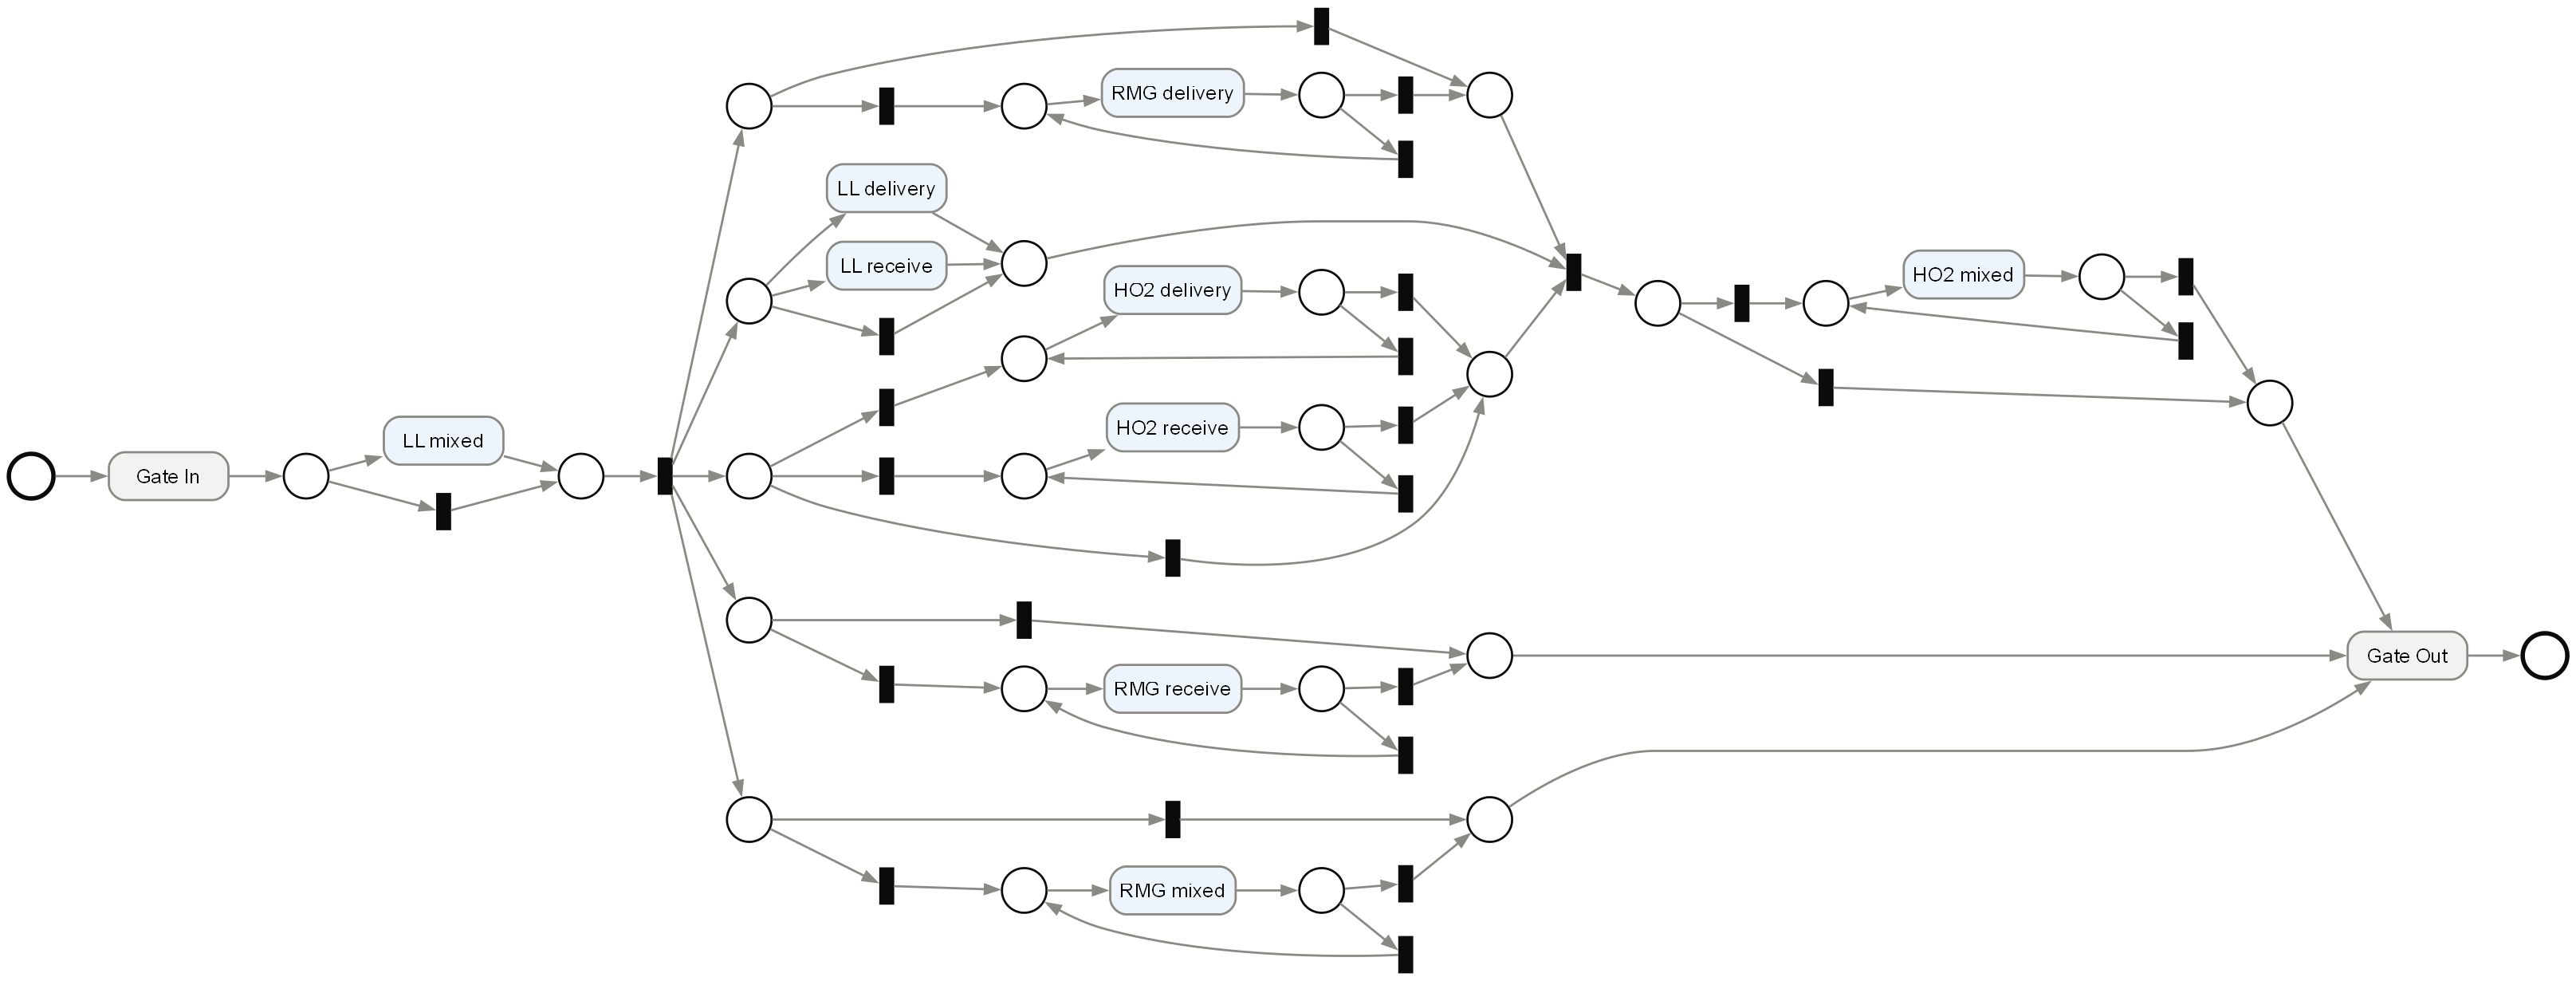
\includegraphics[width=\textwidth,height=0.4\textheight,keepaspectratio]{figures/discovery_prom/net_IM_0.0.png}
\caption{IM 0.0 as discovered (28 places, 11 visible and 27 silent transitions).
Its parallel branches let several stops be enabled at once; silent transitions
skip the branches.}
\label{fig:app_net_im}
\end{figure}

\begin{figure}[htbp]
\centering
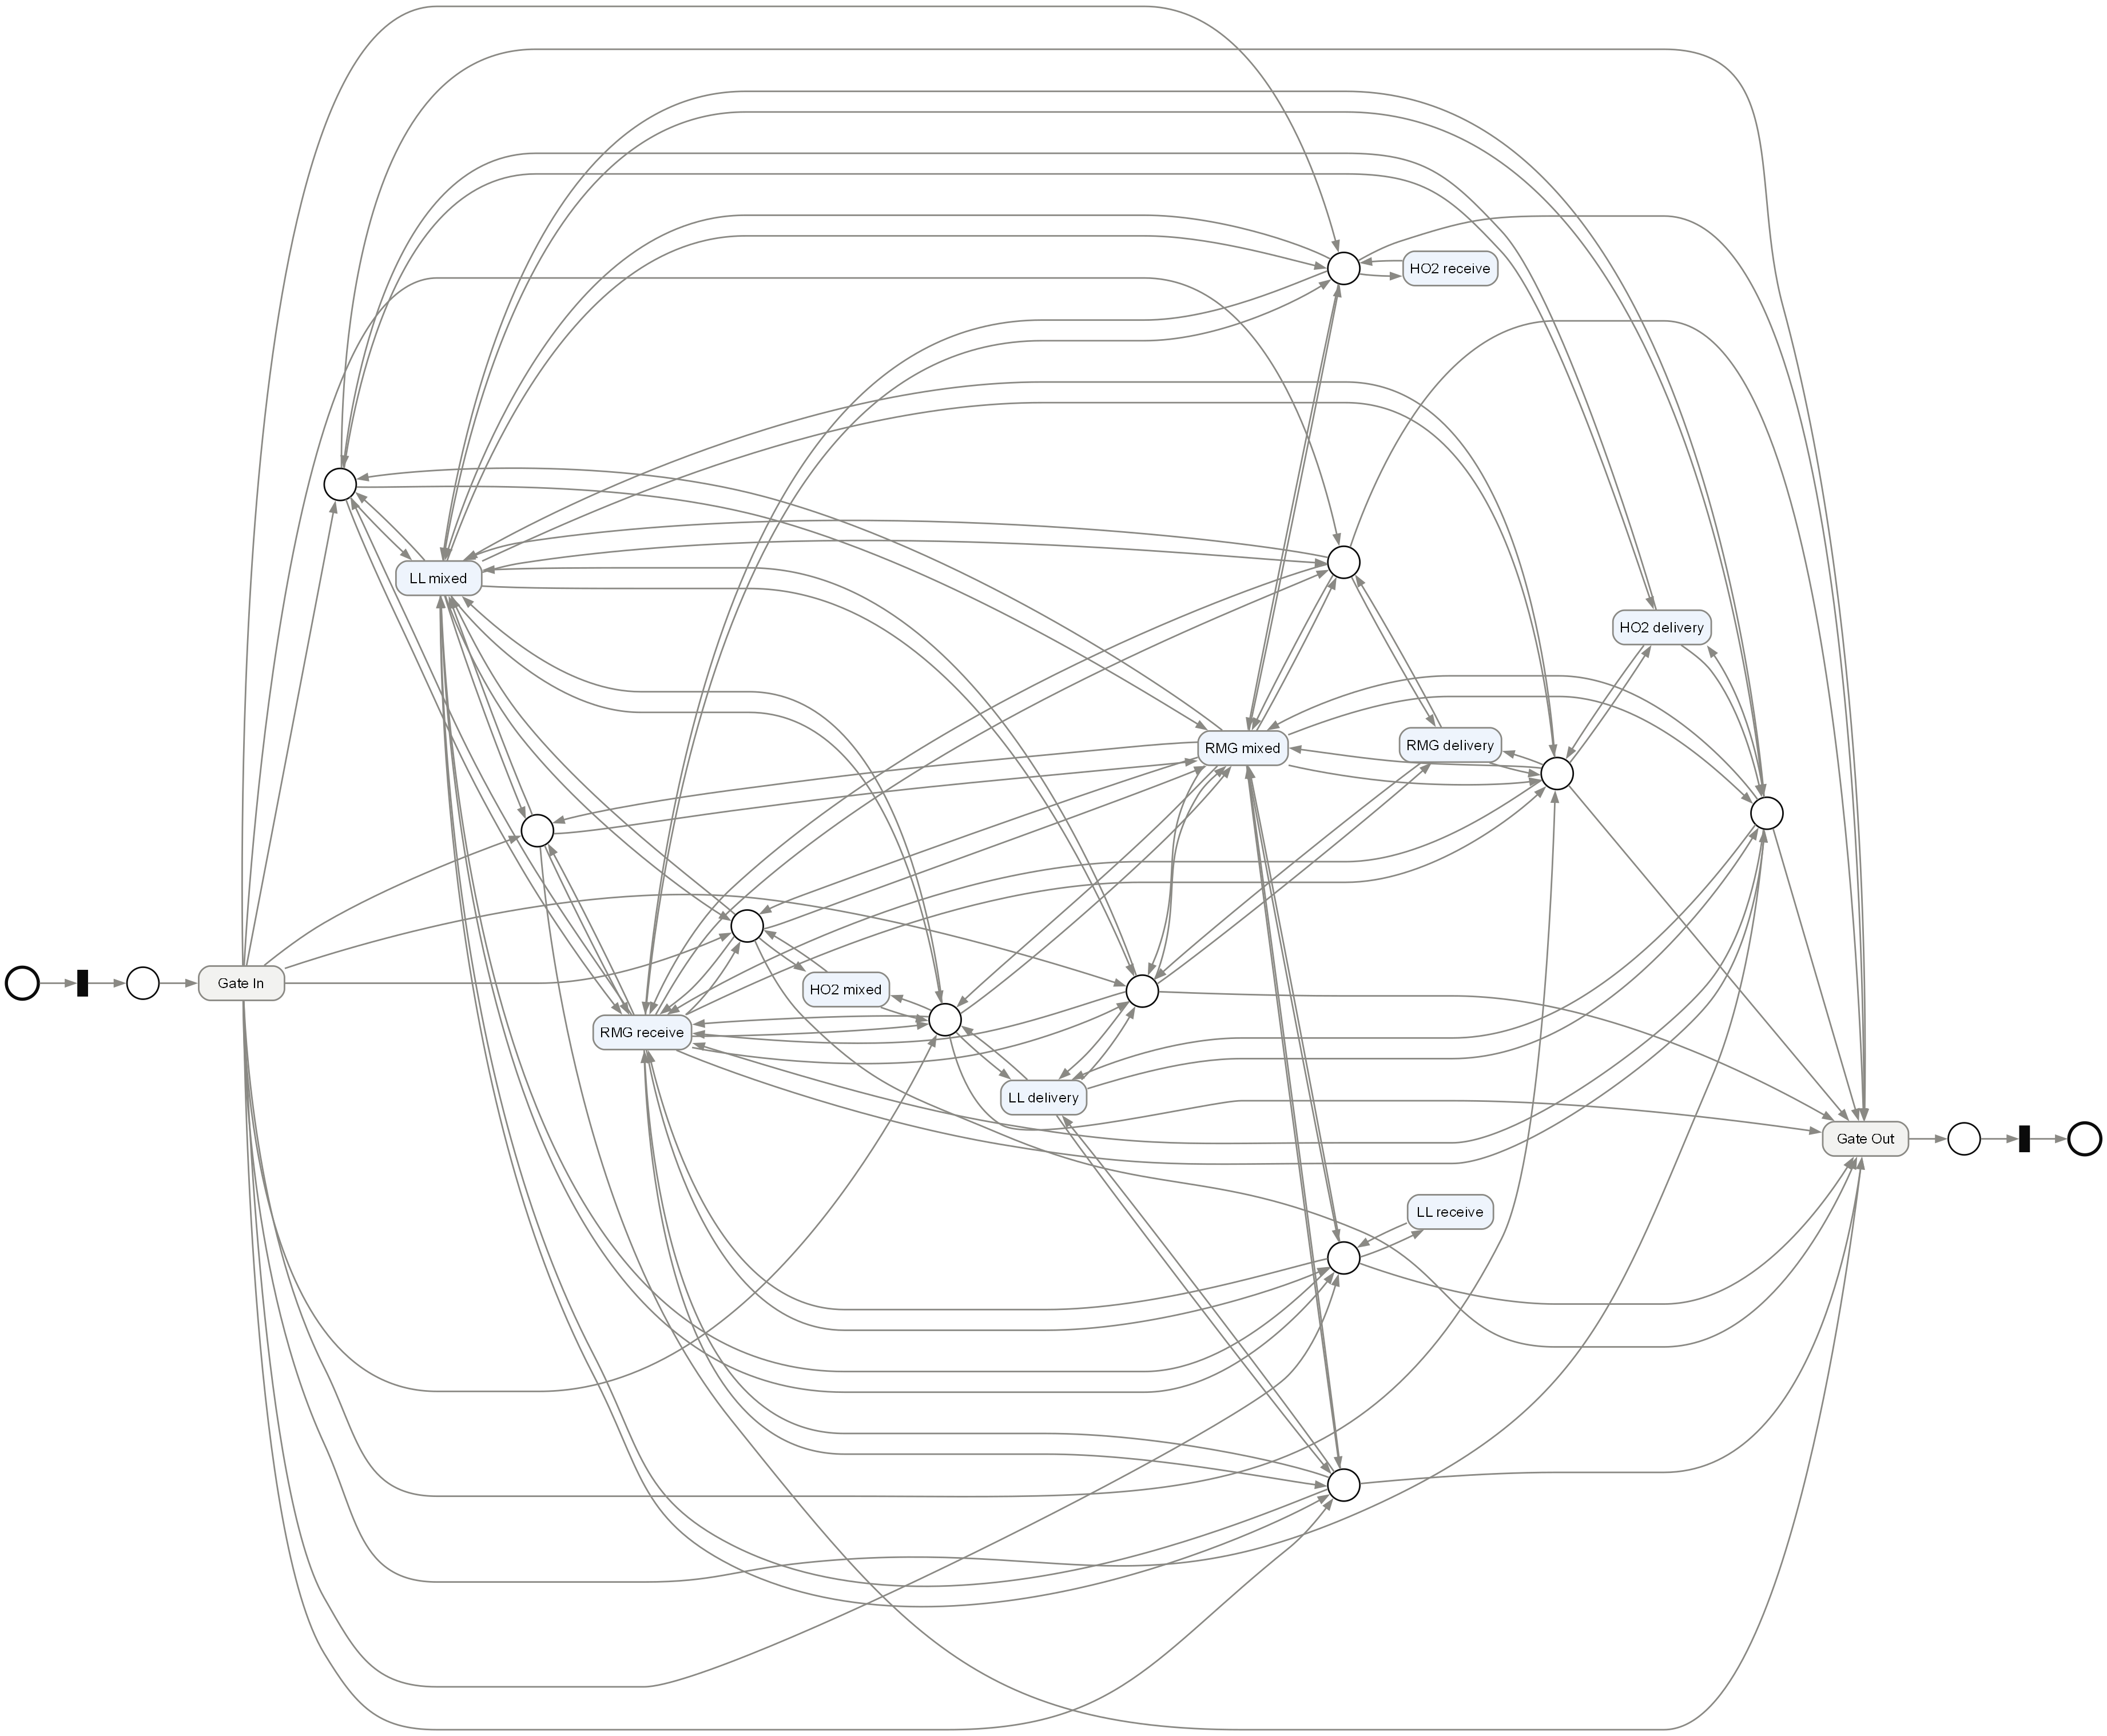
\includegraphics[width=\textwidth,height=0.4\textheight,keepaspectratio]{figures/discovery_prom/net_ILP_1.00.png}
\caption{ILP 1.00 as discovered (15 places, 11 visible and 2 silent transitions).}
\label{fig:app_net_ilp}
\end{figure}

\begin{figure}[htbp]
\centering
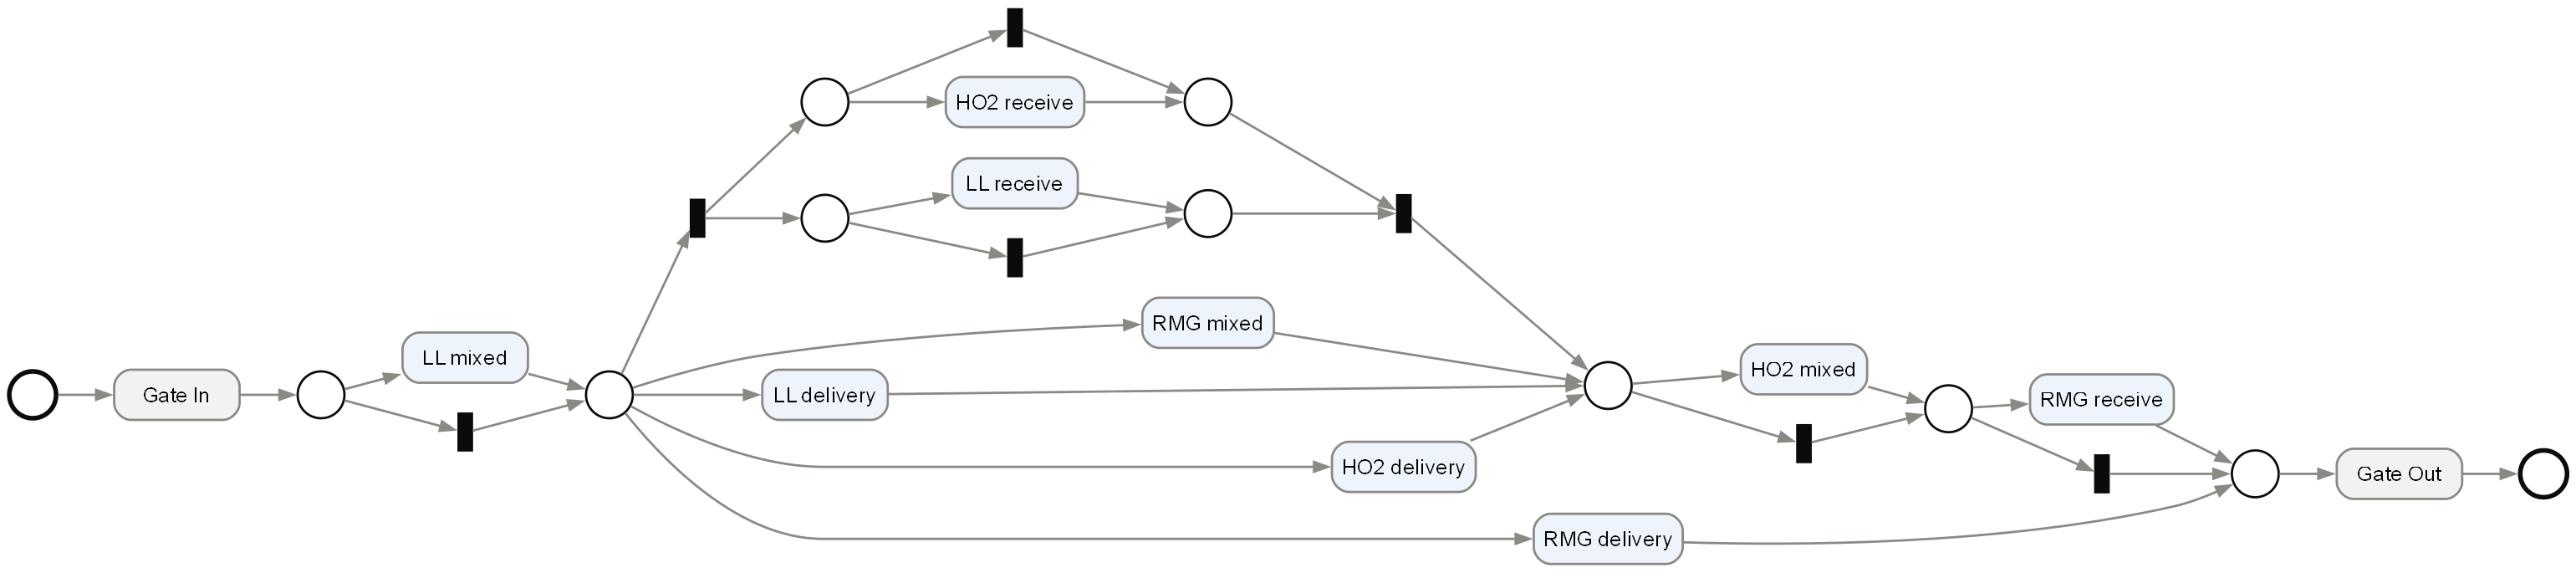
\includegraphics[width=\textwidth,height=0.4\textheight,keepaspectratio]{figures/discovery_prom/net_IMf_0.3.png}
\caption{IMf 0.3 as discovered (11 places, 11 visible and 7 silent transitions).}
\label{fig:app_net_imf}
\end{figure}

\begin{figure}[htbp]
\centering
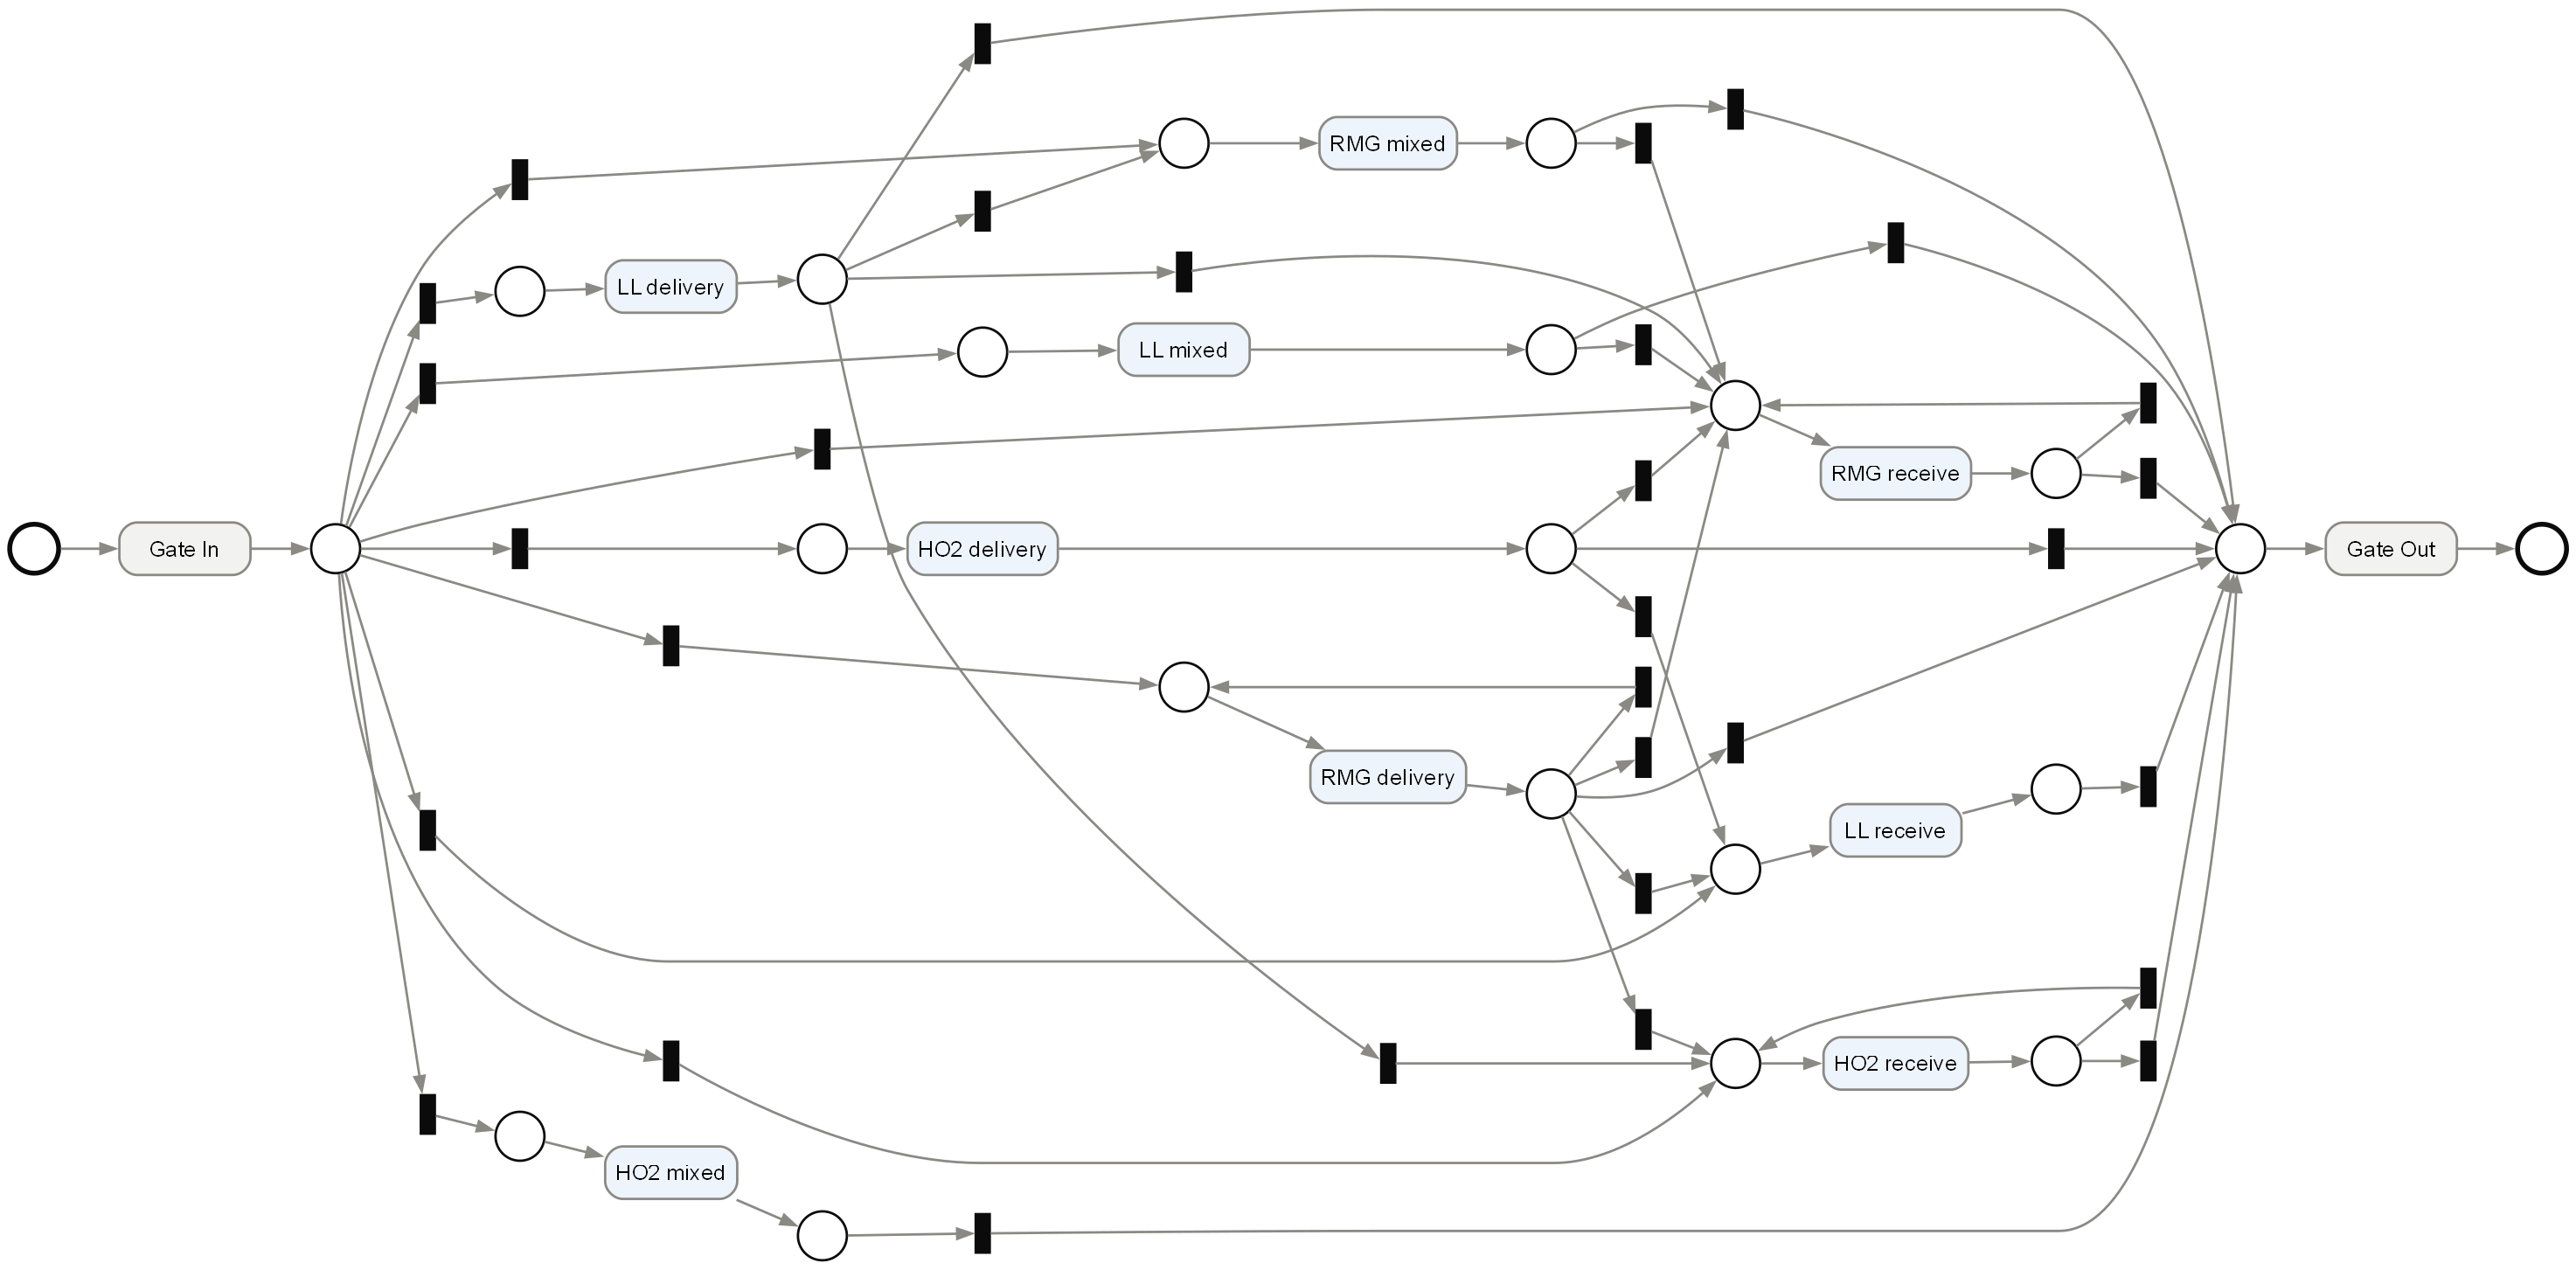
\includegraphics[width=\textwidth,height=0.4\textheight,keepaspectratio]{figures/discovery_prom/net_HM_0.8.png}
\caption{HM 0.8 as discovered (22 places, 11 visible and 31 silent transitions).
It lacks the dependencies from an LL stop to an RMG stop that HM 0.7 has.}
\label{fig:app_net_hm08}
\end{figure}
